%%% lorem.tex --- 
%% 
%% Filename: lorem.tex
%% Description: 
%% Author: Ola Leifler
%% Maintainer: 
%% Created: Wed Nov 10 09:59:23 2010 (CET)
%% Version: $Id$
%% Version: 
%% Last-Updated: Wed Nov 10 09:59:47 2010 (CET)
%%           By: Ola Leifler
%%     Update #: 2
%% URL: 
%% Keywords: 
%% Compatibility: 
%% 
%%%%%%%%%%%%%%%%%%%%%%%%%%%%%%%%%%%%%%%%%%%%%%%%%%%%%%%%%%%%%%%%%%%%%%
%% 
%%% Commentary: 
%% 
%% 
%% 
%%%%%%%%%%%%%%%%%%%%%%%%%%%%%%%%%%%%%%%%%%%%%%%%%%%%%%%%%%%%%%%%%%%%%%
%% 
%%% Change log:
%% 
%% 
%% RCS $Log$
%%%%%%%%%%%%%%%%%%%%%%%%%%%%%%%%%%%%%%%%%%%%%%%%%%%%%%%%%%%%%%%%%%%%%%
%% 
%%% Code:

\chapter{Method}
\label{cha:method}

\section{Pre-processing}
The data for this project was delivered by Östgötatrafiken. The whole dataset is over 300GB in size. The data contains, among other things, GPS coordinates and different types of events representing actions performed by a bus. To be able to feed the data into our models, preprocessing had to be done. The initial data exploration was performed by using jupyter notebooks and the python pandas package. Data operations such filtering and plotting the statistical distributions of the raw data provided an initial overview of the data set. By creating a simple finite state-machine, the data covering a complete journey from a specific bus line could be extracted.


\subsection{Data structure}
The provided data consists of 90 files, where each file represents one day of data. Each file has an approximate size of 5GB. Within the data there are over 20 event-types that represent the state of a bus during a day. For this project four types of events were used, while the others were discarded. The four events used are:
\begin{description}
\item[ObservedPositionEvent:] Gets triggered every second, contains the GPS data of a given bus.
\item[EnteredEvent:] Gets triggered when the bus is within a certain distance to a bus-station. Is used to split the journey into segments.
\item[JourneyStartedEvent:] Gets triggered when the bus is assigned a new journey. Is used to determine which line a bus is currently serving.
\item[JourneyCompletedEvent:] Gets triggered when the bus has completed a journey. Is used as a flag to determine when a journey has ended.
\end{description}

TODO (this section) For this project XXXX bus lines were selected: a subset of the bus line three and bus line number eleven. Line three has been used as a basis, since we all know that bus and we could assure that there were no irregularities on that line. Line eleven had been chosen because it captures a lot of problems that need to be taken into consideration within our predictions. Such problems are GPS variance due to high buildings, high red light density, and sharp corners. 

\subsection{Detecting Segments}
Bus journeys are split into several segments. The \textit{EnteredEvent} is used to detect when a bus is approaching a station, and is also used to split the raw data into segments. The first segment of a journey starts when a \textit{JourneyStartedEvent} triggers. When all the journeys of interest have been collected from the raw data, the collection is investigated in order to find and remove severe anomalies (such as drivers taking a wrong turn). These faulty journeys are discarded since it is not feasible to create a model which takes such complexity into consideration, given the amount of training data available.

\section{Artificial Neural Networks}
The neural network models were made using \textit{Keras} on top of \textit{Tensorflow}. They will be referenced by their notebook name.

\subsection{ANN Model 1}
First, a model was created based on the structure described by (blabla et al, Brazil pappret). With the 

\subsubsection{Model 1v1}
This version of the model predicts the time it takes to travel the current segment. It is assumed that the time is known when the bus left the latest station. The idea is then to subtract the time that has passed since the bus left the latest station from the predicted travel time of the segment to produce a prediction for time left until the bus arrived at the next station.
Features used consists of

%    \item Segment number (one-hot-encoded)}
%    \item Time of day (hour) normalized and (decircled)<- bättre ord tack?
%    \item Time traveld until current segment.


\subsubsection{Model 1v2}
This model was created to be compared with \textit{Version 1}. It was created with all available features from the data. The features include

\begin{itemize}
    \item Segment number (one-hot-encoded)  
\end{itemize}
  
%    \item Time of day (hour) normalized and (decircled)<- bättre ord tack?
%    \item Time traveld until current segment.
%    \item Direction of the bus
%    \item Speed of the bus
%    \item position of the bus

\subsection{ANN Model 2}


%This model predicts the time it will take to travel to the next bus stop. As input this model use time of day normalized to a value in the range [0,1] and the segment for which the observation has been made. The segment input is one-hot encoded meaning that there is an input for each segment in the journey which all have a value of 0 except for the segment of the observation which has the value 1. The network has one fully connected hidden layer with 13 nodes and an output layer with one node. 
%The network uses the \textit{relu} activation function. This model predicts the time in seconds it will take to travel the whole segment. To get a prediction of the time to the next bus stop you need to subtract the actual known time travelled since the previous bus stop from the output of the neural network.

\subsection{Kalman filter}



\section{Gaussian Processes regression for trajectory data}
This section presents how trajectory based GP regression is used to predict the arrival times. The core concept is that each trajectory $x_i$ is considered a realisation of a GP $f^{(i)}(x)$, and when predicting the arrival time of a new trajectory the model computes which GPs it has previously observed that best explain the new data according. However, there are some hurdles with this approach, since trajectories by nature are not synchronised and thus hard to compare in a meaningful way. This was solved by synchronising the trajectories using a separate GP before making the actual predictions. The remainder of this chapter will present in more detail the two steps of synchronisation and prediction.

\subsection{Synchronisation}
As previously mentioned, the trajectories cannot be compared spatially. This is because the buses do not drive \textit{precisely} the same route every time, which can be because of traffic, weather conditions and road work, to mention a few reasons. To be able to train a model on this data the trajectories had to be mapped onto a synchronised space $\tau = [0, 1]$ where they can be compared meaningfully. This was done by training a GP for a synchronising function $f^{(r,s)}_s(x, y)$ for each route $r$ and segment $s$ on a hand picked trajectory. There are two hurdles with this though. Firstly, the data contains a lot of subsegments with buses standing still, which unevenly distributes the data spatially, making the model prioritise getting said subsegments right. Secondly, a GP model does not guarantee that it models a smooth mapping, which is a critical property for this application. To solve the issue of buses standing still, a technique we call \textit{stop compression} is used, and to force the GP to model a smooth mapping \textit{support data} is added. These two issues and techniques used to solve them are described in more detail in the following correspondin subsection.

\subsubsection{Stop Compression}
Since all buses produce at least one data point every second, a lot of clustered data points is generated when a bus stands still on a parking lot before a journey or when encountering a red-light. The GPs that was used assumed a fixed lenghtscale, which came with the assumption that the data was uniformely distributed.
\begin{figure}[H]
  \begin{subfigure}[b]{0.5\textwidth}
    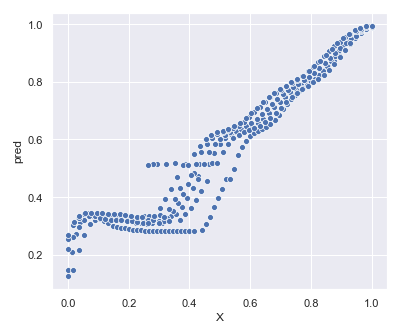
\includegraphics[width=\textwidth]{figures/traj-without-stop-compression.png}
    \caption{Estimated trajectory progression for new data without stop compression.}
    \label{fig:progression-without-stop-compression}
  \end{subfigure}
  %
  \begin{subfigure}[b]{0.5\textwidth}
    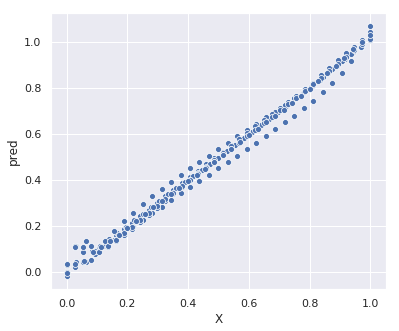
\includegraphics[width=\textwidth]{figures/traj-with-stop-compression.png}
    \caption{Estimated trajectory progression for new data with stop compression.}
    \label{fig:progression-with-stop-compression}
  \end{subfigure}
\end{figure}
This assumption is no good with several points clustered on the same spot, so to make the assumption reasonable, all the data points generated during a stand-still were clustered into one with the mean values of all clustered points. Without this compression, the trajectory used to learn $f^{(r,s)}_s$ also mattered a lot, since where it stopped during a journey would greatly affect the estimated synchronisation function. As shown in figures~\ref{fig:progression-without-stop-compression} and~\ref{fig:progression-without-stop-compression}, the estimated trajectory progression with stop compression much more closely resemble the actual progression, indicated by the linear relationship.

\subsubsection{Support Data}
In addition to requiring the data to be uniformly distributed, it was essential that $f^{(r,s)}_s$ was a smooth mapping with respect to the direction of spatial progress; that is, data points close in spatial progression should be mapped onto points in $\tau$ which are also close by. Furthermore, data distributed orthogonally to the direction of spatial progression should be mapped onto the same point in $\tau$. This requirement is quite reasonable when you concider that a bus driving slightly more to the left on a road is no closer to its destination than a bus driving slightly more to the right. Another motivation for this is that the GPS data includes some measurement error which has to be considered in the synchronisation.

\begin{figure}[H]
  \begin{subfigure}[b]{0.5\textwidth}
    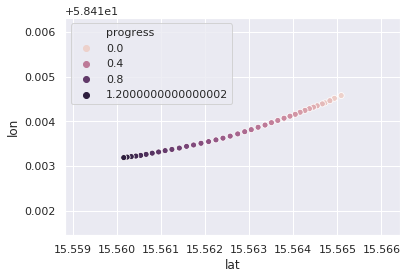
\includegraphics[width=\textwidth]{figures/traj-without-support-data.png}
    \caption{Spatial progression of trajectory 2.}
    \label{fig:traj-without-support-data}
  \end{subfigure}
  %
  \begin{subfigure}[b]{0.5\textwidth}
    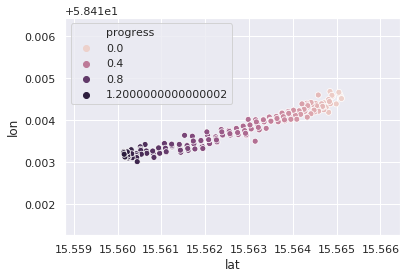
\includegraphics[width=\textwidth]{figures/traj-with-support-data.png}
    \caption{Spatial progression of support data 2.}
    \label{fig:traj-with-support-data}
  \end{subfigure}
\end{figure}

In order to force the GP to model a function with this property, each data point $d^{(i)}$ was duplicated by placing a normal distribution over it, orthogonal to the spatial progression vector ${(d^{(i+1)}_x - d^{(i)}_x, d^{(i+1)}_y - d^{(i)}_y)}^T$, and drawing several samples with the same progression as $d^{(i)}$. This process is illustrated in figures~\ref{fig:traj-without-support-data} and~\ref{fig:traj-with-support-data}. The generated support data was saved to a separate data set and combined with the trajectory data when training synhronisation GPs.

\begin{figure}[H]
  \begin{subfigure}[b]{0.5\textwidth}
    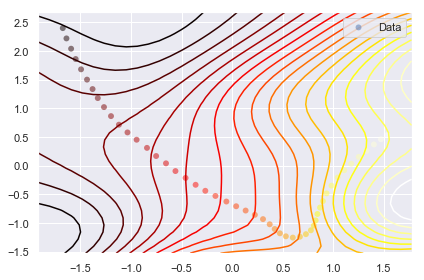
\includegraphics[width=\textwidth]{figures/heat-without-support-data.png}
    \caption{Heightmap of a synchronisation GP without using support data.}
    \label{fig:heightmap-without-support}
  \end{subfigure}
  %
  \begin{subfigure}[b]{0.5\textwidth}
    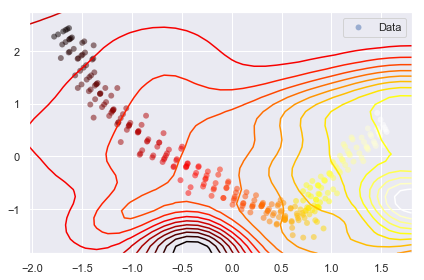
\includegraphics[width=\textwidth]{figures/heat-with-support-data.png}
    \caption{Heightmap of a synchronisation GP using support data.}
    \label{fig:heightmap-with-support}
  \end{subfigure}
\end{figure}

As shown in figures~\ref{fig:heightmap-without-support} and~\ref{fig:heightmap-with-support}, using support data greatly increase the smoothness of $f^{(r,s)}_s$, and which contours are orthogonal to the spatial progression.

%%%%%%%%%%%%%%%%%%%%%%%%%%%%%%%%%%%%%%%%%%%%%%%%%%%%%%%%%%%%%%%%%%%%%%
%%% lorem.tex ends here

%%% Local Variables: 
%%% mode: latex
%%% TeX-master: "demothesis"
%%% End: 
